The main interaction mode of \nusmv is through an interactive shell.
In this mode \nusmv enters a read-eval-print loop. The user can
activate the various \nusmv computation steps as system commands with
different options. These steps can therefore be invoked separately,
possibly undone or repeated under different modalities. These steps
include the construction of the model under different partitioning
techniques, model checking of specifications, and the configuration of
the BDD package. The interactive shell of \nusmv is activated from the
system prompt as follows ('\nusmvprompt' is the default \nusmv
shell prompt):

\begin{alltt}
\shellprompt \shelltext{\nusmvtxt -int} \ret
\nusmvprompt
\end{alltt}

A \nusmv command is a sequence of words. The first word specifies the
command to be executed. The remaining words are arguments to the
invoked command. Commands separated by a `\code{;}' are executed
sequentially; the \nusmv shell waits for each command to terminate in
turn. The behavior of commands can depend on environment variables,
similar to \csh environment variables.

In the following we present the possible commands followed by the
related environment variables, classified in different
categories. Every command answers to the option \commandopt{h} by
printing out the command usage. When output is paged for some commands
(option \commandopt{m}), it is piped through the program specified by
the \unix \shellvar{PAGER} shell variable, if defined, or through the
\unix command \shellcommand{more}. Environment variables can be
assigned a value with the \shellcommand{set} command.  Command
sequences to \nusmv must obey the (partial) order specified in the
figure depicted on page \pageref{flowchart}. For instance, it is not
possible to evaluate CTL expressions before the model is built.

A number of commands and environment variables, like those dealing
with file names, accept arbitrary strings. There are a few reserved
characters which must be escaped if they are to be used literally in
such situations. See the section describing the \command{history}
command, on page \pageref{History Command}, for more information.\\

The verbosity of \nusmv is controlled by the following environment
variable.

\begin{nusmvVar} {verbose\_level}{\range{0}{4}}{\natnum{0}}
Controls the verbosity of the system. Possible values are integers from
\varvalue{0} (no messages) to \varvalue{4} (full messages). The
default value is \varvalue{0}.
\end{nusmvVar}

\section{Model Reading and Building}
\index{model reading}
\index{model parsing}
\index{model compiling}
The following commands allow for the parsing and compilation of the
model into a BDD.

\input{cmd/read_model}

\begin{nusmvVar} {input\_file}{\filename{input\_file}}{none}
Stores the name of the input file containing the
model. It can be set by the \shellcommand{set} command or by the command
line option `{\it -i}'. There is no default value.
\end{nusmvVar}

\begin{nusmvVar} {pp\_list}{\code{pps}}{none}
Stores the list of pre-processors to be run on the input file before
it is parsed by \nusmv. The pre-processors are executed in the order
specified by this variable. The argument must either be the empty
string (specifying that no pre-processors are to be run on the input
file), one single pre-processor name or a space seperated list of
pre-processor names inside double quotes. Any invalid names are
ignored. The default is none.
\end{nusmvVar}

\begin{nusmvCommand} {flatten\_hierarchy} {Flattens the hierarchy of modules}

\cmdLine{flatten\_hierarchy [-h]}

This command is responsible of the instantiation of modules and
processes. The instantiation is performed by substituting the actual
parameters for the formal parameters, and then by prefixing the result
via the instance name.

\end{nusmvCommand}


\begin{nusmvCommand}{show\_vars} {Shows model's symbolic variables and their values}

\cmdLine{show\_vars [-h] [-s] [-i] [-m | -o output-file]}

Prints symbolic input and state variables of the model with their
range of values (as defined in the input file).

\begin{cmdOpt}

\opt{-s}{Prints only state variables.}

\opt{-i}{Prints only input variables.}

\opt{-m}{Pipes the output to the program specified by the
\shellvar{PAGER} shell variable if defined, else through the
\unix command \shellcommand{more}.}

\opt{-o \parameter{\filename{output-file}}}{Writes the output generated by the command to
\filename{output-file}.}

\end{cmdOpt}

\end{nusmvCommand}


\input{cmd/encode_variables}

\begin{nusmvVar} {input\_order\_file}{\filename{input\_order\_file}}{none}
Indicates the file name containing the variable ordering to be used in
building the model by the `\command{encode\_variables}' command. There
is no default value.
\end{nusmvVar}

\begin{nusmvVar} {write\_order\_dumps\_bits}{none}{none}
Changes the behaviour of the command \command{write\_order}. 

When this variable is set, \command{write\_order} will dump the bits
constituting the boolean encoding of each scalar variable, instead of
the scalar variable itself. This helps to work at bits level in the
variable ordering file. See the command \command{write\_order} for
further information. The default value is \varvalue{0}. 
\end{nusmvVar}

\input{cmd/write_order}

\begin{nusmvVar} {output\_order\_file}{\filename{output\_order\_file}}{\filename{temp.ord}}
The file where the current variable ordering has to be written. The default value is
`\filename{temp.ord}'. \index{\filename{temp.ord}}
\end{nusmvVar}

\input{cmd/build_model}

\begin{nusmvVar} {partition\_method}{\set{Method}{Monolithic, Threshold, Iwls95CP}}{none}
The method to be used in building the transition relation, and to
compute images and preimages. Possible values are:

\begin{itemize}
\item {\varvalue{\bf Monolithic}}. No partitioning at all.

\item {\varvalue{\bf Threshold}}. Conjunctive partitioning, with a simple
threshold heuristic. Assignments are collected in a single cluster
until its size grows over the value specified in the variable
\varName{conj\_part\_threshold}. It is possible (default) to use affinity
clustering to improve model checking performance. See
\varName{affinity} variable.

\item {\varvalue{\bf Iwls95CP}}. Conjunctive partitioning, with clusters generated and
ordered according to the heuristic described in~\cite{RAP+95}. Works
in conjunction with the variables \varName{image\_cluster\_size},
\varName{image\_W1}, \varName{image\_W2}, \varName{image\_W3}, \varName{image\_W4}.
It is possible (default) to use affinity clustering to improve model 
checking performance. See \varName{affinity} variable. It is also possible
to avoid (default) preordering of clusters (see~\cite{RAP+95}) by
setting the \varName{iwls95preorder} variable appropriately.
\end{itemize}

\end{nusmvVar}

\begin{nusmvVar}{conj\_part\_threshold}{\natnum{Number}}{\natnum{0}}
The limit of the size of clusters in conjunctive partitioning. The
default value is \varvalue{0} BDD nodes.
\end{nusmvVar}

\begin{nusmvVar} {affinity}{\set{value}{0, 1}}{\natnum{1}}
Enables affinity clustering heuristic described in \cite{MOON00},
possible values are \varvalue{0} or \varvalue{1}. The default value is \varvalue{1}.
\end{nusmvVar}

% \begin{nusmvVar} {image\_cluster\_size, image\_W\{1,2,3,4\}}
% The parameters to configure the behavior of the \Iwls partitioning
% algorithm.  \varName{image\_cluster\_size} is used as threshold value
% for the clusters. The default value is \varvalue{1000} BDD nodes. The
% other parameters attribute different weights to the different factors
% in the algorithm. The default values are \varvalue{6}, \varvalue{1},
% \varvalue{1}, \varvalue{2} respectively. (For a detailed description,
% please refer to \cite{RAP+95}.)
% \end{nusmvVar}
% SPLIT INTO SEPERATE ENTRIES:

\begin{nusmvVar}{image\_cluster\_size}{\natnum{Number}}{\natnum{1000}}
One of the parameters to configure the behaviour of the \Iwls
partitioning algorithm. \varName{image\_cluster\_size} is used as
threshold value for the clusters. The default value is \varvalue{1000}
BDD nodes.
\end{nusmvVar}

\begin{nusmvVar}{image\_W\{1,2,3,4\}}{\natnum{Number}}{\natnum{\{6,1,1,2\}}}
The other parameters for the \Iwls partitioning algorithm. These
attribute different weights to the different factors in the
algorithm. The default values are \varvalue{6}, \varvalue{1},
\varvalue{1}, \varvalue{6} respectively. (For a detailed description,
please refer to \cite{RAP+95}.)
\end{nusmvVar}

\begin{nusmvVar} {iwls95preorder}{\set{value}{0,1}}{\natnum{0}}
Enables cluster preordering following heuristic described in
\cite{RAP+95}, possible values are \varvalue{0} or \varvalue{1}. The
default value is \varvalue{0}. Preordering can be very slow.
\end{nusmvVar}

\begin{nusmvVar} {image\_verbosity}{\set{value}{0,1}}{\natnum{0}}
Sets the verbosity for the image method \Iwls, possible values
are \varvalue{0} or \varvalue{1}. The default value is \varvalue{0}.
\end{nusmvVar}

\input{cmd/print_iwls95options}
\begin{nusmvCommand} {go} {Initializes the system for the verification.}

\cmdLine{go [-h]}

This command initializes the system for verification. It is equivalent
to the command sequence \command{read\_model},
\command{flatten\_hierarchy}, \command{encode\_variables}, \linebreak
\command{build\_model}, \command{build\_flat\_model},
\command{build\_boolean\_model}.  If some commands have already been
executed, then only the remaining ones will be invoked.

\end{nusmvCommand}

\begin{nusmvCommand}{process\_model} {Performs the batch steps and then returns control to the interactive shell.}

\cmdLine{process\_model [-h] [-i model-file] [-m Method]}

Reads the model, compiles it into BDD and performs the model checking
of all the specification contained in it. If the environment variable
\envvar{forward\_search} has been set before, then the set of
reachable states is computed. If the environment variables
\envvar{enable\_reorder} and \envvar{reorder\_method} are set, then
the reordering of variables is performed accordingly. This command
simulates the batch behavior of \nusmv and then returns the control to
the interactive shell.

\begin{cmdOpt}
 
\opt{-i \parameter{\filename{model-file}}}{Sets the environment variable
\envvar{input\_file} to file \filename{model-file}, and reads the
model from file \filename{model-file}.}
 
\opt{-m \parameter{\set{Method}{Monolithic, Threshold, Iwls95CP}}}{Sets the environment variable
\envvar{partition\_method} to \code{Method} and uses it as
partitioning method.}

\end{cmdOpt}
\end{nusmvCommand}


\section{Commands for Checking Specifications}
The following commands allow for the BDD-based model checking of a
\nusmv model.

\begin{nusmvCommand}{compute\_reachable} {Computes the set of reachable states}

\cmdLine{compute\_reachable [-h]}

Computes the set of reachable states. The result is then used to
simplify image and preimage computations. This can result in improved
performances for models with sparse state spaces. Sometimes this
option may slow down the performances because the computation of
reachable states may be very expensive. The environment variable
\envvar{forward\_search} is set during the execution of this
command.

\end{nusmvCommand}

\begin{nusmvCommand}{print\_reachable\_states} {Prints out the number of reachable states}

\cmdLine{print\_reachable\_states [-h] [-v]}

Prints the number of reachable states of the given model. In verbose
mode, prints also the list of all reachable states.  The reachable
states are computed if needed.

\end{nusmvCommand}

\input{cmd/check_fsm}

\begin{nusmvVar} {check\_fsm}{\set{value}{0,1}}{\natnum{0}}
Controls the activation of the totality check of the transition relation
during the \linebreak \command{process\_model} call. Possible values are \varvalue{0} or
\varvalue{1}. Default value is \varvalue{0}.
\end{nusmvVar}
%  [[[ ROVERI .  If the transition relation is not total then a potential
% deadlock state is printed. This checking is performed by computing
% @emph{(not(EX(reachable_states)) and INVAR)} if the result of such a
% computation is the set of deadlock states.  The reachable states are
% computed before, in order to ensure that the deadlock states are
% actually reachable.  ]]]

\input{cmd/print_fair_states}
\input{cmd/print_fair_transitions}

\begin{nusmvCommand}{check\_spec} {Performs fair CTL model checking.}

\cmdLine{check\_spec [-h] [-m | -o output-file] [-n number | -p \linebreak"\ctlexpr [IN context]"]}

Performs fair CTL model checking.

A \ctlexpr to be checked can be specified at command line using
option \commandopt{p}. Alternatively, option \commandopt{n} can be
used for checking a particular formula in the property database. If
neither \commandopt{n} nor \commandopt{p} are used, all the SPEC
formulas in the database are checked.\\
\begin{cmdOpt}

\opt{-m}{Pipes the output generated by the command in processing
\code{SPEC}s to the program specified by the \shellvar{PAGER} shell
variable if defined, else through the \unix command
\shellcommand{more}.}

\opt{-o \parameter{\filename{output-file}}}{Writes the output generated by the command in
processing \code{SPEC}s to the file \filename{output-file}.}
            
\opt{-p \parameter{"\ctlexpr [IN context]"}}{A CTL formula to be checked.
\code{context} is the module instance name which the variables in
\ctlexpr must be evaluated in.}

\opt{-n \parameter{\natnum{number}}}{Checks the CTL property with index \natnum{number} in
the property database.} 

\end{cmdOpt}
  If the \envvar{ag\_only\_search} environment variable has been set,
  then a specialized algorithm to check AG formulas is used instead of
  the standard model checking algorithms.
\end{nusmvCommand}


\begin{nusmvVar} {ag\_only\_search}{\set{value}{0,1}}{\natnum{0}}
Enables the use of an ad hoc algorithm for checking AG formulas.
Given a formula of the form \formula{AG alpha}, the algorithm computes
the set of states satisfying \formula{alpha}, and checks whether it
contains the set of reachable states. If this is not the case, the
formula is proved to be false.
\end{nusmvVar}

\begin{nusmvVar} {forward\_search}{\set{value}{0,1}}{\natnum{0}}
Enables the computation of the reachable states during the
\command{process\_model} command and when used in conjunction with the
\envvar{ag\_only\_search} environment variable enables the use of an ad hoc
algorithm to verify invariants.
\end{nusmvVar}

\begin{nusmvCommand} {check\_invar} {Performs model checking of invariants}
 
 \cmdLine{check\_invar [-h] [-m | -o output-file] [-n number | -p
 \linebreak "\invarexpr [IN context]"]}
 
Performs invariant checking on the given model. An invariant is a set
of states. Checking the invariant is the process of determining that
all states reachable from the initial states lie in the invariant.
Invariants to be verified can be provided as simple formulas (without
any temporal operators) in the input file via the \code{INVARSPEC}
keyword or directly at command line, using the option \commandopt{p}.
   
Option \commandopt{n} can be used for checking a particular invariant
of the model. If neither \commandopt{n} nor \commandopt{p} are used,
all the invariants are checked.
  
During checking of invariant all the fairness conditions associated
with the model are ignored.
  
If an invariant does not hold, a proof of failure is demonstrated.
This consists of a path starting from an initial state to a state
lying outside the invariant. This path has the property that it is the
shortest path leading to a state outside the invariant.

\begin{cmdOpt}

\opt{-m}{Pipes the output generated by the program in processing
  \code{INVARSPEC}s to the program specified by the \shellvar{PAGER}
  shell variable if defined, else through the \unix command
\shellcommand{more}.}
 
\opt{-o \parameter{\filename{output-file}}}{Writes the output
  generated by the command in processing \code{INVARSPEC}s to the file
  \filename{output-file}.}
            
\opt{-p \parameter{"\invarexpr [IN context]"}}{The command line
  specified invariant formula to be verified.  \code{context} is the
  module instance name which the variables in  \invarexpr must be
  evaluated in.}

\end{cmdOpt}

\end{nusmvCommand}

\input{cmd/check_ltlspec}
\begin{nusmvCommand}{compute} {Performs computation of quantitative characteristics}

\cmdLine{compute [-h] [-m | -o output-file] [-n number | -p \linebreak"compute-expr [IN context]"]}

This command deals with the computation of quantitative
characteristics of real time systems. It is able to compute the length
of the shortest (longest) path from two given set of states.
\begin{center}
\code{MAX [ alpha , beta ]} \\
\code{MIN [ alpha , beta ]} 
\end{center}
Properties of the above form can be specified in the input file via
the keyword \code{COMPUTE} or directly at command line, using option
\commandopt{p}.

Option \commandopt{n} can be used for computing a particular
expression in the model. If neither \commandopt{n} nor \commandopt{p}
are used, all the COMPUTE specifications are computed.

\begin{cmdOpt}

\opt{-m}{Pipes the output generated by the command in processing
\code{COMPUTE}{s} to the program specified by the \shellvar{PAGER} shell
variable if defined, else through the \unix command
\shellcommand{more}.}

\opt{-o \parameter{\filename{output-file}}}{Writes the output generated by the command in
processing \code{COMPUTE}{s} to the file \filename{output-file}.}

\opt{-p \parameter{"\compexpr [IN context]"}}{A COMPUTE formula to be checked.
\code{context} is the module instance name which the variables in
\compexpr must be evaluated in.}

\opt{-n \parameter{\natnum{number}}}{Computes only the property with index \natnum{number}.}

\end{cmdOpt}
\end{nusmvCommand}

\input{cmd/add_property}

\section{Commands for Bounded Model Checking}
\label{Commands for Bounded Model Checking}
\index{Commands for Bounded Model Checking} 

In this section we describe in detail the commands for doing and
controlling Bounded Model Checking in \nusmv.  Bounded Model Checking
is based on the reduction of the bounded model checking problem to a
propositional satisfiability problem. After the problem is generated,
\nusmv internally calls a propositional SAT solver in order to find an
assignment which satisfies the problem.  Currently \nusmv supplies
three SAT solvers: \SIM, \zchaff and \minisat.  \zchaffminisatnotice
They are therefore not included in the source code distribution or in
some of the binary distributions of \nusmv.

Some commands for Bounded Model Checking use incremental algorithms.
These algorithms exploit the fact that satisfiability
problems generated for a particular bounded model checking problem
often share common subparts. So information obtained during solving of
one satisfiability problem can be used in solving of
another one. The incremental algorithms usually run quicker then
non-incremental ones but require a SAT solver with incremental
interface. At the moment, only \zchaff and \minisat offer such an
interface.  If none of these solvers are linked to \nusmv, then the
commands which make use of the incremental algorithms will not be available.

It is also possible to generate the satisfiability problem without
calling the SAT solver. Each generated problem is dumped in
\dimacs format to a file. \dimacs is the standard format used as input
by most SAT solvers, so it is possible to use \nusmv with a separate
external SAT solver. At the moment, the \dimacs files can be generated only by
commands which do not use incremental algorithms.

\input{cmd/bmc_setup}
\begin{nusmvCommand} {go\_bmc} {Initializes the system for the BMC verification.}

\cmdLine{go\_bmc [-h]}

This command initializes the system for verification. It is equivalent
to the command sequence \command{read\_model},
\command{flatten\_hierarchy}, \command{encode\_variables}, \linebreak
\command{build\_boolean\_model}, \command{bmc\_setup}.  If some
commands have already been executed, then only the remaining ones will
be invoked.

\end{nusmvCommand}

\input{cmd/check_ltlspec_bmc}
\input{cmd/check_ltlspec_bmc_onepb}
\input{cmd/gen_ltlspec_bmc}
\input{cmd/gen_ltlspec_bmc_onepb}
\input{cmd/check_ltlspec_bmc_inc}

\begin{nusmvVar} {bmc\_length}{\natnum{Number}}{\natnum{10}}
Sets the generated problem bound. Possible values are any natural
number, but must be compatible with the current value held by the
variable \emph{bmc\_loopback}. The default value is \varvalue{10}.
\end{nusmvVar}

\begin{nusmvVar} {bmc\_loopback}{\set{loop}{\range{0}{bmc\_length-1},
\range{-1}{-bmc\_length}, X, *}}{*}
Sets the generated problem loop. Possible values are: 

\begin{itemize}
\item Any natural number, but less than the current value of
the variable \emph{bmc\_length}. In this case the loop point is absolute.
\item Any negative number, but greater than or equal to
-\emph{bmc\_length}. In this case specified loop is the loop length. 
\item The symbol '\varvalue{X}', which means ``no loopback".
\item The symbol '\varvalue{*}', which means ``any possible loopbacks".
\end{itemize}

The default value is \varvalue{*}.
\end{nusmvVar}

\begin{nusmvVar} {bmc\_dimacs\_filename}{\filename{bmc\_dimacs\_filename}}{\filename{@f\_k@k\_l@l\_n@n.dimacs}}
This is the default file name used when generating \dimacs problem
dumps. This variable may be taken into account by all commands which
belong to the gen\_ltlspec\_bmc family.  \dimacs file name can contain
special symbols which will be expanded to represent the actual file
name. Possible symbols are:

\begin{itemize}
\item {\bf @F}
The currently loaded model name with full path. 
\item {\bf @f}
The currently loaded model name without path part. 
\item {\bf @n}
The numerical index of the currently processed formula in the property
database.
\item {\bf @k} 
The currently generated problem length. 
\item {\bf @l}
The currently generated problem loopback value.   
\item {\bf @@}
The `@' character.   
\end{itemize}

The default value is ``\filename{@f\_k@k\_l@l\_n@n}".
\end{nusmvVar}

\input{cmd/check_invar_bmc}

\input{cmd/gen_invar_bmc}

\input{cmd/check_invar_bmc_inc}

\begin{nusmvVar} {bmc\_invar\_alg}
{\set{invariant proving algorithm}{classic, een-sorensson}}{classic}
Sets the default algorithm used by the command \code{check\_invar\_bmc}. 
Possible values are \varvalue{classic} and \varvalue{een-sorensson}.
The default value is \varvalue{classic}.
\end{nusmvVar}

\begin{nusmvVar} {bmc\_inc\_invar\_alg}
{\set{invariant proving incremental algorithm}{dual, zigzag}}{dual}
Sets the default algorithm used by the command \code{check\_invar\_bmc\_inc}. 
Possible values are \code{dual} and \code{zigzag}.
The default value is \varvalue{dual}.
\end{nusmvVar}

\begin{nusmvVar} {bmc\_invar\_dimacs\_filename}{\filename{bmc\_invar\_dimacs\_filename}}{\filename{@f\_invar\_n@n.dimacs}}
This is the default file name used when generating \dimacs invar
dumps. This variable may be taken into account by the command
\command{gen\_invar\_bmc}.  \dimacs file name can contain special symbols which will
be expanded to represent the actual file name. Possible symbols are:
\begin{itemize}
\item {\bf @F}
The currently loaded model name with full path. 
\item {\bf @f}
The currently loaded model name without path part. 
\item {\bf @n}
The numerical index of the currently processed formula in the properties
database.
\item {\bf @@}
The `@' character.   
\end{itemize}
The default value is ``\filename{@f\_invar\_n@n}".\\
\end{nusmvVar}

\begin{nusmvVar} {sat\_solver}{\set{SAT Solver}{\SIM, \zchaff, \minisat}}{\SIM}
The SAT solver's name actually to be used. Default SAT solver is \SIM.
Depending on the \nusmv configuration, also the \zchaff and \minisat
SAT solvers can be available or not. \zchaffminisatnotice
\end{nusmvVar}

\begin{nusmvCommand}{bmc\_simulate} {Generates a trace of the model from 0 (zero) to k}

\cmdLine{bmc\_simulate [-h | -k ]}

\command{bmc\_simulate} does not require a specification to build the
problem, because only the model is used to build it.  The problem
length is represented by the \commandopt{k} command parameter, or by
its default value stored in the environment variable
\envvar{bmc\_length}.

\begin{cmdOpt}
\opt{-k \parameter{\natnum{\it length}}}{ {\it length} is the length of the generated
simulation.}
\end{cmdOpt}

\end{nusmvCommand}



\section{Commands for checking PSL specifications}
\label{Commands for checking PSL specifications}
\index{Commands for checking PSL specifications}

The following command allow for model checking of PSL specifications.

\input{cmd/check_pslspec}


\section{Simulation Commands}
\label{Simulation Commands}
\index{ Simulation Commands}

In this section we describe the commands that allow to simulate a
\nusmv specification. See also the section \sref{Traces} that
describes the commands available for manipulating traces.

\input{cmd/pick_state}

\begin{nusmvVar} {showed\_states}{\range{1}{100}}{\natnum{25}}
Controls the maximum number of states showed during an interactive
simulation session. Possible values are integers from
\varvalue{1} to \varvalue{100}. The default value is \varvalue{25}.
\end{nusmvVar}

\input{cmd/simulate}

\section{Traces}
\label{Traces}
\index{Traces}
%
A trace is a sequence of states-inputs pairs corresponding to a
possible execution of the model. Each pair contains the inputs that
caused the transition to the new state, and the new state itself. The
initial state has no such input values defined as it does not depend
on the values of any of the inputs. The values of any constants
declared in \texttt{DEFINE} sections are also part of a trace. If the
value of a constant depends only on state variables then it will be
treated as if it is a state variable too. If it depends only on input
variables then it will be treated as if it is an input variable. If
however, a constant depends upon both input and state variables, then
it gets displayed in a seperate ``combinatorial'' section. Since the
values of any such constants depend on one or more inputs, the initial
state does not contain this section either.\\

Traces are created by \nusmv when a formula is found to be false; they
are also generated as a result of a simulation (\sref{Simulation
Commands}).  Each trace has a number, and the states-inputs pairs are
numbered within the trace.  Trace {\it n} has states/inputs {\it n.1,
n.2, n.3, "..."} where \textit{n.1} represents the initial state.\\

\subsection{Inspecting Traces}
\label{Inspecting Traces}
\index{ Inspecting Traces}
%
The trace inspection commands of \nusmv allow for navigation along the
labelled states-inputs pairs of the traces produced. During the
navigation, there is a {\it current state}, and the {\it current
trace} is the trace the {\it current state} belongs to. The commands
are the following:

\begin{nusmvCommand} {goto\_state} {Goes to a given state of a trace}

\cmdLine{goto\_state [-h] state\_label}

Makes \code{state\_label} the \emph{current state}. This command is used to
navigate along traces produced by \nusmv. During the navigation, there
is a \emph{current state}, and the \emph{current trace} is the trace
the \emph{current state} belongs to.

\end{nusmvCommand}

\input{cmd/print_current_state}


\subsection{Displaying Traces}
\label{Displaying Traces}
\index{ Displaying Traces}
%
\nusmv comes with three trace plugins (see \sref{Trace Plugins}) which
can be used to display traces in the system. Once a trace has been
generated by \nusmv it is printed to \texttt{stdout} using the trace
explanation plugin which has been set as the current default. The
command \command{show\_traces} (see \sref{Simulation Commands}) can
then be used to print out one or more traces using a different trace
plugin, as well as allowing for output to a file.


\subsection{Trace Plugin Commands}
\label{Trace Plugin Commands}
\index{ Trace Plugin Commands}
The following commands relate to the plugins which are available
in \nusmv.

\input{cmd/show_plugins}

\begin{nusmvVar} {default\_trace\_plugin}{\range{0}{5}}{\natnum{0}}
This determines which trace plugin will be used by default when traces
that are generated by \nusmv are to be shown. The values that this
variable can take depend on which trace plugins are installed. Use the
command
\command{show\_plugins} to see which ones are available. The default
value is \varvalue{0}.
\end{nusmvVar}

\begin{nusmvCommand} {show\_traces} {Shows the traces generated in a \nusmvhead session}

\cmdLine{show\_traces [-h] [-v] [-t] [-m | -o output-file] [-p plugin-no]
    \linebreak {[-a | trace\_number]}}

Shows the traces currently stored in system memory, if any. By default
it shows the last generated trace, if any.

\begin{cmdOpt}
\opt{-v} { Verbosely prints traces content (all state variables,
otherwise it prints out only those variables that have changed their
value from previous state). This option only applies when the Basic
Trace Explainer plugin is used to display the trace.}

\opt{-t}{ Prints only the total number of currently stored traces.}

\opt{-a}{ Prints all the currently stored traces.}

\opt{-m}{ Pipes the output through the program specified by the
\shellvar{PAGER} shell variable if defined, else through the \unix
command \shellcommand{more}.}

\opt{-o \parameter{\filename{output-file}}}{Writes the output generated by the command to
\filename{output-file}.}

\opt{-p \parameter{\natnum{plugin-no}}}{Uses the specified trace
  plugin to display the trace.}

\opt{\natnum{trace\_number}}{ The (ordinal) identifier number of the trace to
 be printed. This must be the last argument of the command. Omitting
 the trace number causes the most recently generated trace to be printed.}
\end{cmdOpt}

If the XML Format Output plugin is being used to save generated traces
to a file with the intent of reading them back in again at a later
date, then only one trace should be saved per file. This is because
the trace reader does not currently support multiple traces in one
file.

\end{nusmvCommand}

\begin{nusmvCommand} {read\_trace} {Loads a previously saved trace}

\cmdLine{read\_trace [-h | -i file-name]}

\begin{cmdOpt}
\opt{-i \parameter{\filename{file-name}}}{ Reads in a trace from the
specified file. Note that the file must only contain one trace.}

\end{cmdOpt}

Loads a trace which has been previously output to a file with the XML
Format Output plugin. The model from which the trace was originally
generated must be loaded and built using the command ``\command{go}''
first.\\Please note that this command is only available on systems
that have the Expat XML parser library installed.
\end{nusmvCommand}



\section{Trace Plugins}
\label{Trace Plugins}
\index{ Trace Plugins}
\nusmv comes with three plugins which can be used to diaplay a trace
that has been generated:

\begin{center}
\begin{tabular}{l}
Basic Trace Explainer\\
States/Variables Table\\
XML Format Printer\\
\end{tabular}
\end{center}

There is also a plugin which can read in any trace which has been
output to a file by the XML Format Printer. Note however that this
reader is only available on systems that have the Expat XML parser
library installed.\\
\\
Once a trace has been generated it is output to \texttt{stdout} using
the currently selected plugin. The command \command{show\_traces} can
be used to output any previuosly generated, or loaded, trace to a
specific file.

\subsection{Basic Trace Explainer}
\label{Basic Trace Explainer}
\index{ Basic Trace Explainer}

This plugin prints out each state (the current values of the
variables) in the trace, one after the other. The initial state
contains all the state variables and their initial values. States are
numbered in the following fasion:

\begin{center}
\texttt{trace\_number.state\_number}
\end{center}

There is the option of printing out the value of every variable in
each state, or just those which have changed from the previous
one. The one that is used can be chosen by selecting the appropriate
trace plugin. The values of any constants which depend on both input
and state variables are printed next. It then prints the set of inputs
which cause the transition to a new state (if the model contains
inputs), before actually printing the new state itself. The set of
inputs and the subsequent state have the same number associated to
them.

In the case of a looping trace, if the next state to be printed is the
same as the last state in the trace, a line is printed stating that
this is the point where the loop begins.

With the exception of the initial state, for which no input values are
printed, the output syntax for each state is as follows:

\begin{alltt}
-> Input: TRACE_NO.STATE_NO <-
    /* for each input var (being printed), i: */
    INPUT_VARi = VALUE
-> State: TRACE_NO.STATE_NO <-
    /* for each state var (being printed), j: */
    STATE_VARj = VALUE
    /* for each combinatorial constant (being printed), k: */
    CONSTANTk = VALUE
\end{alltt}

where \texttt{INPUT\_VAR}, \texttt{STATE\_VAR} and \texttt{CONSTANT}
have the relevant module names prepended to them (seperated by a
period) with the exception of the module ``\texttt{main}'' .

The version of this plugin which only prints out those variables whose
values have changed is the initial default plugin used by \nusmv.


\subsection{States/Variables Table}
\label{States/Variables Table}
\index{ States/Variables Table}

This trace plugin prints out the trace as a table, either with the
states on each row, or in each column. The entries along the state
axis are:

\begin{center}
\texttt{S0 C1 I1 S1 ...~Cn In Sn}
\end{center}

where \texttt{S0} is the initial state, and \texttt{$I_i$} gives the
values of the input variables which caused the transition from state
\texttt{$S_{i-1}$} to state \texttt{$S_i$}. \texttt{$C_i$} gives the
values of any combinatorial constants, where the value depends on the
values of the state variables in state \texttt{$S_{i-1}$} and the
values of input variables in state \texttt{$S_i$}.

The variables in the model are placed along the other axis. Only the
values of state variables are displayed in the State row/column, only
the values of input variables are displayed in the Input row/column
and only the values of combinatorial constants are displayed in the
Constants row/column. All remaining cells have '\texttt{-}' displayed.


\subsection{XML Format Printer}
\label{XML Format Printer}
\index{ XML Format Printer}

This plugin prints out the trace either to \texttt{stdout} or to a
specified file using the command \command{show\_traces}.  If traces
are to be output to a file with the intention of them being loaded
again at a later date, then each trace must be saved in a separate
file. This is because the XML Reader plugin does not currently support
multiple traces per file.\\The format of a dumped XML trace file is as
follows:

\begin{alltt}
<?XML_VERSION_STRING?>
<counter-example type=TRACE_TYPE desc=TRACE_DESC>

  /* for each state, i: */
  <node>
    <state id=i>

      /* for each state var, j: */
      <value variable=j>VALUE</value>

    </state>
    <combinatorial id=i+1>

      /* for each combinatorial constant, k: */
      <value variable=k>VALUE</value>

    </combinatorial>
    <input id=i+1>

      /* for each input var, l: */
      <value variable=l>VALUE</value>

    </input>
  </node>

</counter-example>
\end{alltt}

Note that for the last state in the trace, there is no input section
in the node tags. This is because the inputs section gives the new
input values which cause the transition to the next state in the
trace. There is also no combinatorial section as this depends on the
values of the inputs and are therefore undefined when there are no
inputs.


\subsection{XML Format Reader}
\label{XML Format Reader}
\index{ XML Format Reader}

This plugin makes use of the Expat XML parser library and as such can
only be used on systems where this library is available. Previously
generated traces for a given model can be loaded using this plugin
provided that the original model file\footnote{To be exact, $M_1
\subseteq M_2$, where $M_1$ is the model from which the trace was
generated, and $M_2$ is the currently loaded, and built, model. Note
however, that this may mean that the trace is not valid for the model
$M_2$.} has been loaded, and built using the command \command{go}.

When a trace is loaded, it is given the smallest available trace
number to identify it. It can then be manipulated in the same way as
any generated trace.


\section{Interface to the DD Package}
\label{Interface to DD package}
\index{interface to DD Package}
\label{DD package interface}
\index{ DD package interface}

\nusmv uses the state of the art BDD package \cudd \cite{Som98}.
Control over the BDD package can very important to tune the
performance of the system. In particular, the order of variables is
critical to control the memory and the time required by operations
over BDDs.  Reordering methods can be activated to determine better
variable orders, in order to reduce the size of the existing BDDs.

Reordering of the variables can be triggered in two ways: by the user,
or by the BDD package.  In the first way, reordering is triggered by
the interactive shell command \command{dynamic\_var\_ordering} with the
\commandopt{f} option.

Reordering is triggered by the BDD package when the number of nodes
reaches a given threshold. The threshold is initialized and
automatically adjusted after each reordering by the package.  This is
called dynamic reordering, and can be enabled or disabled by the
user.  Dynamic reordering is enabled with the shell command
\command{dynamic\_var\_ordering} with the option \commandopt{e}, and disabled
with the \commandopt{d} option. 


\begin{nusmvVar} {enable\_reorder}{\set{value}{0,1}}{\natnum{0}}
Specifies whether dynamic reordering is enabled (when value is `\varvalue{0}')
or disabled (when value is `\varvalue{1}').
\end{nusmvVar}

\begin{nusmvVar} {reorder\_method}{\set{Method}{sift, random, random\_pivot,
sift\_converge, symmetry\_sift, symetry\_sift\_converge,
window\{2,3,4\}, window\{2,3,4\}\_converge, group\_sift,
group\_sift\_converge, annealing, genetic, exact, linear, linear\_converge}}{sift}
Specifies the ordering method to be used when dynamic variable
reordering is fired. The possible values, corresponding to the
reordering methods available with the \cudd package, are listed below.
The default value is \varvalue{sift}. 

\begin{supertabular}{lp{210pt}}
\opt{\varvalue{sift}:} {
Moves each variable throughout the order to find an optimal position for
that variable (assuming all other variables are fixed). This generally
achieves greater size reductions than the window method, but is slower.}

\opt{\varvalue{random}:}{
Pairs of variables are randomly chosen, and swapped in the order. The
swap is performed by a series of swaps of adjacent variables. The best
order among those obtained by the series of swaps is retained. The
number of pairs chosen for swapping equals the number of variables in
the diagram.}

\opt{\varvalue{random\_pivot}:}{
Same as \varvalue{random}, but the two variables are chosen so that the
first is above the variable with the largest number of nodes, and the
second is below that variable. In case there are several variables tied
for the maximum number of nodes, the one closest to the root is used.}

\opt{\varvalue{sift\_converge}:}{
The \varvalue{sift} method is iterated until no further improvement is
obtained.}

\opt{\varvalue{symmetry\_sift}:}{
This method is an implementation of symmetric sifting. It is similar to
sifting, with one addition: Variables that become adjacent during
sifting are tested for symmetry. If they are symmetric, they are linked
in a group. Sifting then continues with a group being moved, instead of
a single variable.}

\opt{\varvalue{symmetry\_sift\_converge}:}{
The \varvalue{symmetry\_sift} method is iterated until no further improvement
is obtained.}

\opt{window\{2,3,4\}:}{
Permutes the variables within windows of {\it n} adjacent variables, where
{\it n} can be either 2, 3 or 4, so as to minimize the overall BDD
size.}

\opt{\varvalue{window\{2,3,4\}\_converge}:}{
The \varvalue{window\{2,3,4\}} method is iterated until no further improvement is
obtained.}

\opt{\varvalue{group\_sift}:}{
This method is similar to \varvalue{symmetry\_sift}, but uses more general
criteria to create groups.}

\opt{\varvalue{group\_sift\_converge}:}{
The \varvalue{group\_sift} method is iterated until no further improvement
is obtained.}

\opt{\varvalue{annealing}:}{
This method is an implementation of simulated annealing for variable
ordering. This method is potentially very slow.}

\opt{\varvalue{genetic}:}{
This method is an implementation of a genetic algorithm for variable
ordering. This method is potentially very slow.}

\opt{\varvalue{exact}:}{
This method implements a dynamic programming approach to exact
reordering. It only stores one BDD at a time. Therefore, it is relatively
efficient in terms of memory. Compared to other reordering strategies,
it is very slow, and is not recommended for more than 16 boolean
variables.}

\opt{\varvalue{linear}:}{
This method is a combination of sifting and linear transformations.}

\opt{\varvalue{linear\_conv}:}{
The \varvalue{linear} method is iterated until no further improvement is obtained.}

\end{supertabular}
\end{nusmvVar}

\input{cmd/dynamic_var_ordering}

\input{cmd/print_bdd_stats}

\input{cmd/set_bdd_parameters}

\section{Administration Commands}
\label{administration commands}
\index{administration commands}

This section describes the administrative commands offered by the
interactive shell of \nusmv.

\begin{nusmvCommand}{!}{shell\_command}
\cindex{"!, \see{bang}}
``\command{!}" executes a shell command. The \shellcommand{shell\_command} is
executed by calling \shellcommand{bin/sh -c {shell\_command}}. If the command
does not exists or you have not the right to execute it, then an error
message is printed.
\end{nusmvCommand}

\input{cmd/alias}
\begin{nusmvCommand}{echo} {Merely echoes the arguments}

\cmdLine{echo [-h] [-o filename [-a]] <string>}

Echoes the specified string either to standard output, or to
\filename{filename} if the option \commandopt{o} is specified.
\begin{cmdOpt}
\opt{-o \parameter{\filename{filename}}} { Echoes to the specified
filename instead of to standard output. If the option \commandopt{a}
is not specified, the file \filename{filename} will be overwritten 
if it already exists. }

\opt{-a} {Appends the output to the file specified by option
\commandopt{o}, instead of overwritting it. Use only with the option 
\commandopt{o}.}
\end{cmdOpt}
\end{nusmvCommand}

\input{cmd/help}
\input{cmd/history}
\input{cmd/print_usage}
\begin{nusmvCommand} {quit} {exits \nusmvhead}
 
\cmdLine{quit [-h] [-s]}

Stops the program.  Does not save the current network before
exiting.\\
\begin{cmdOpt}
\opt{-s}{ Frees all the used memory before quitting.  This is slower,
and it is used for finding memory leaks.}
\end{cmdOpt}
\end{nusmvCommand}

\input{cmd/reset}
\input{cmd/set}
\input{cmd/source}
\input{cmd/time}
\input{cmd/unalias}

\newpage
\input{cmd/unset}

\input{cmd/usage}

\input{cmd/which}

\section{Other Environment Variables}
\label{Shell configuration Variables}
\index{ Shell configuration Variables}
%
The behavior of the system depends on the value of some environment
variables. For instance, an environment variable specifies the
partitioning method to be used in building the transition relation.  The
value of environment variables can be inspected and modified with the
\shellcommand{set} command. Environment variables can be either logical
or utility.

\begin{nusmvVar} {autoexec}{<command string>}{none}
Defines a command string to be automatically executed after every
command processed by the command interpreter. This may be useful for
timing commands, or tracing the progress of optimization.
\end{nusmvVar}

\begin{nusmvVar} {on\_failure\_script\_quits}{none}{none}
When a non-fatal error occurs during the interactive mode, the
interactive interpreter simply stops the currently executed command,
prints the reason of the problem, and prompts for a new command.  When
set, this variables makes the command interpreter quit when an error
occur, and then quit \nusmv. This behaviour might be useful when the
command \command{source} is controlled by either a system pipe or
a shell script. Under these conditions a mistake within the script
interpreted by \command{source} or any unexpected error might
hang the controlling script or pipe, as by default the interpreter
would simply give up the current execution, and wait for further
commands. 
The default value of this environment variable is \varvalue{0}.
\end{nusmvVar}


\begin{nusmvVar}{filec}{\set{value}{on,off}}{off}
Enables file completion a la \csh.  If the system has been compiled
with the \nusmvreadline library, the user is able to perform file
completion by typing the \tab key (in a way similar to the file
completion inside the \bash shell). If the system has not been
compiled with the \nusmvreadline library, a built-in method to perform
file completion a la \csh can be used. This method is enabled with
the `\command{set filec}' command. The \csh file completion method can
be also enabled if the \nusmvreadline library has been used. In this case
the features offered by \nusmvreadline will be disabled.
\end{nusmvVar}

\begin{nusmvVar}{shell\_char}{<any character>}{!}
\envvar{shell\_char} specifies a character to be used as shell escape.
The default value of this environment variable is `\varvalue{!}'.
\end{nusmvVar}

\begin{nusmvVar} {history\_char}{<any character>}{\%}
\envvar{history\_char} specifies a character to be used in history
substitutions.
The default value of this environment variable is `\varvalue{\%}'.
\end{nusmvVar}

\begin{nusmvVar} {open\_path}{<path names>}{none}
\code{open\_path} (in analogy to the shell-variable \shellvar{PATH}) is a
list of colon-separated strings giving directories to be searched
whenever a file is opened for read. Typically the current directory
(\code{.}) is first in this list. The standard system library
(\stdsyslib) \vindex{\stdsyslib}
is always implicitly appended to the current path. This provides a
convenient short-hand mechanism for reaching standard library files.
\end{nusmvVar}

\begin{nusmvVar} {nusmv\_stderr}{\filename{stderr\_file}}{none}
Standard error (normally \code{stderr}) can be re-directed to a file
by setting the variable \envvar{nusmv\_stderr}.
\end{nusmvVar}

\begin{nusmvVar} {nusmv\_stdout}{\filename{stdout\_file}}{none}
Standard output (normally \code{stdout}) can be re-directed to a file
by setting the internal variable \envvar{nusmv\_stdout}.
\end{nusmvVar}

\begin{nusmvVar} {nusmv\_stdin}{\filename{stdin\_file}}{none}
Standard input (normally \code{stdin}) can be re-directed to a file
by setting the internal variable \envvar{nusmv\_stdin}.
\end{nusmvVar}

\begin{figure}[t]
\label{flowchart}
\begin{center}
%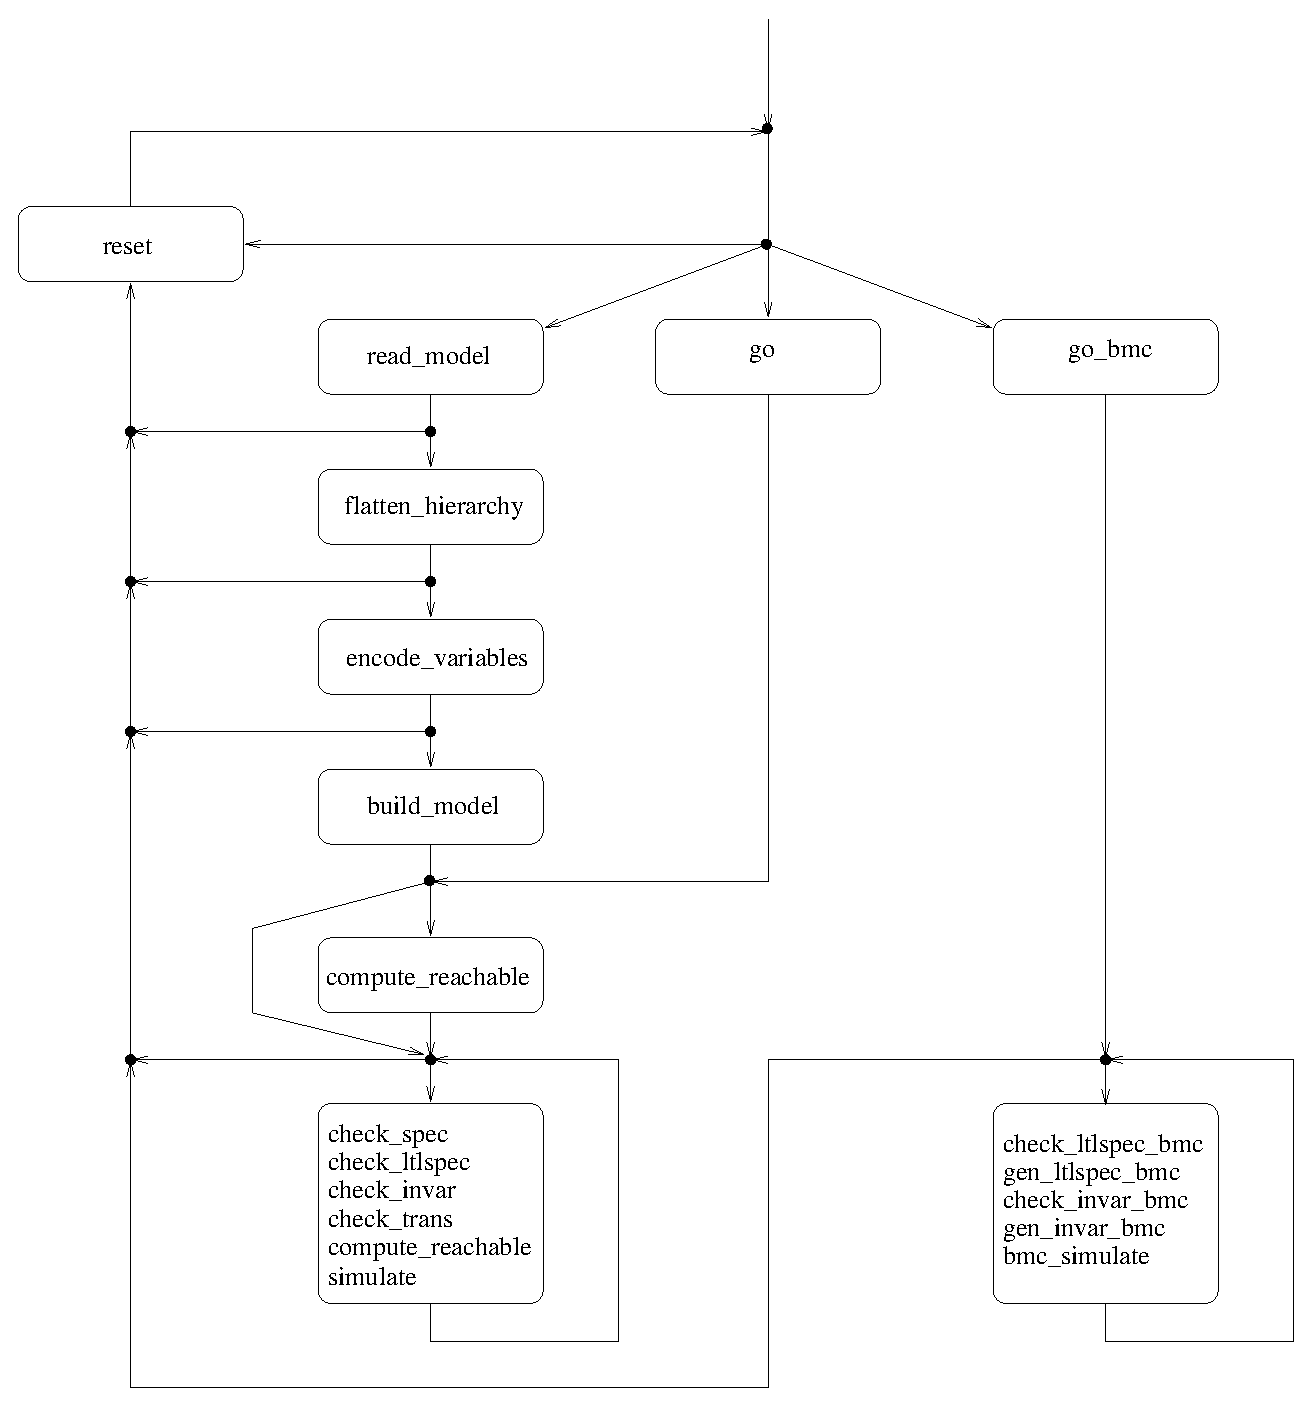
\includegraphics[width=0.8\textwidth]{cmdpo}
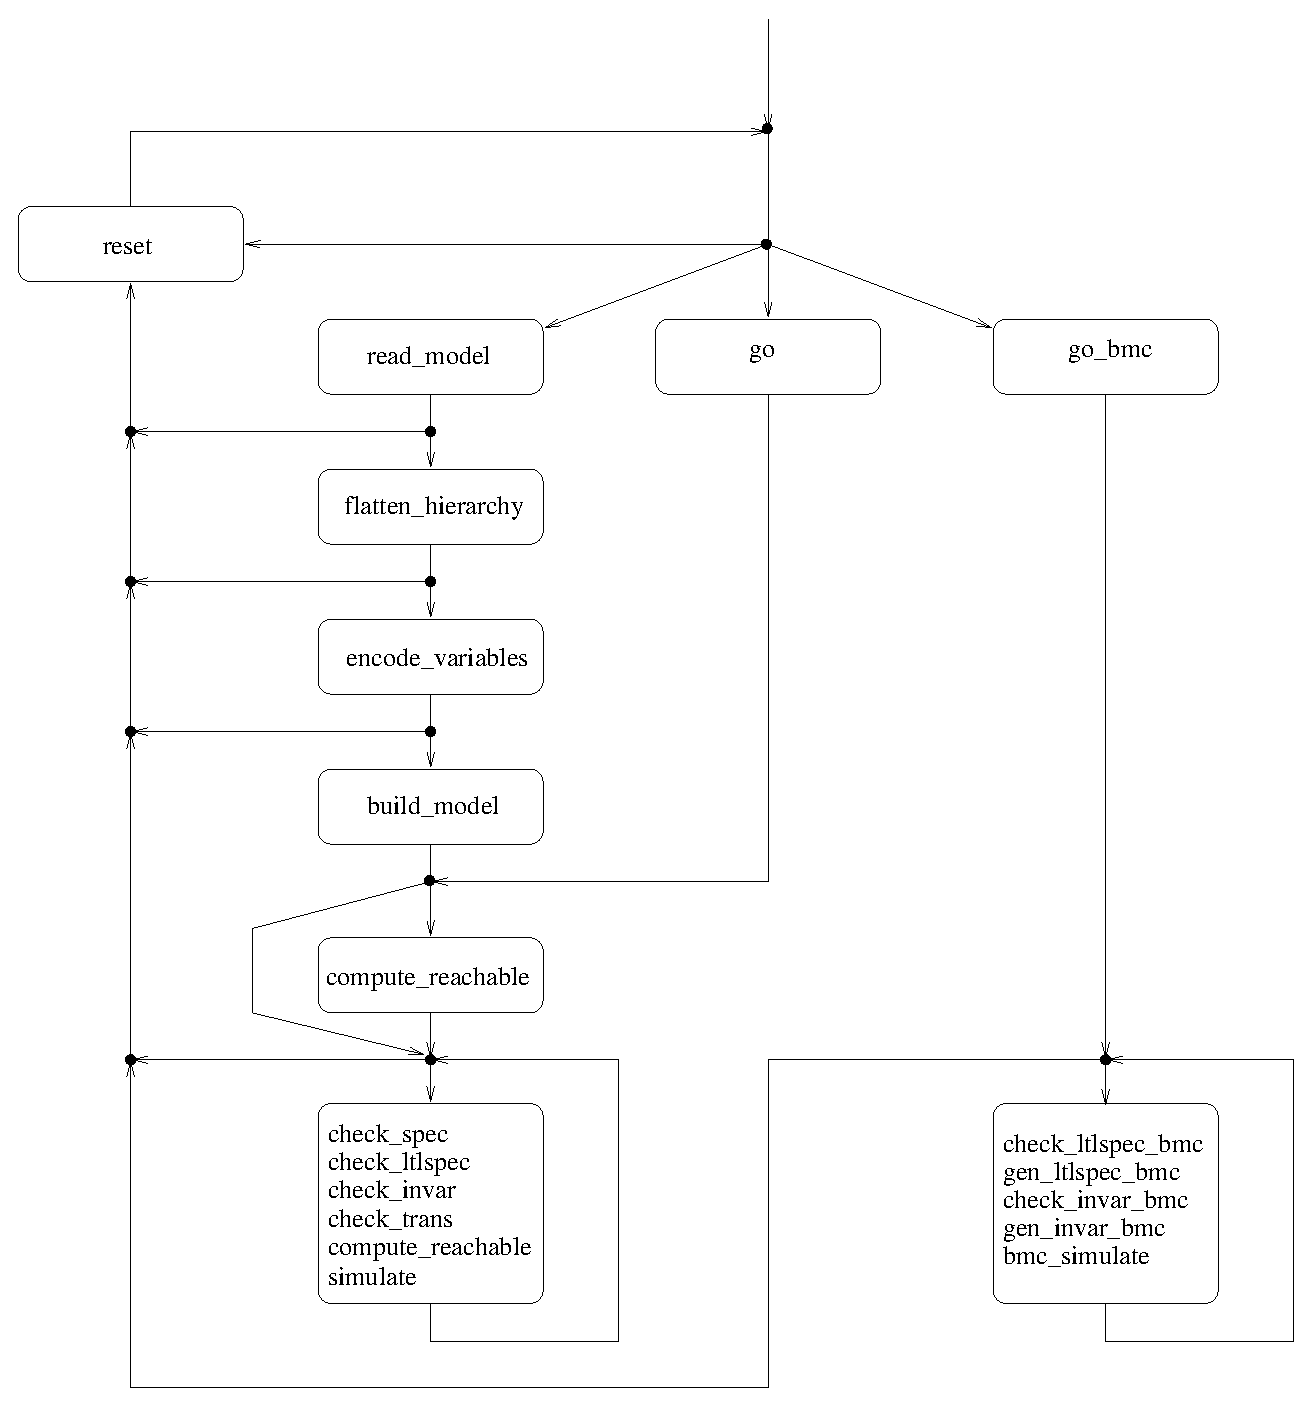
\includegraphics[width=\textwidth]{cmdpo}
\caption{The dependency among \nusmv commands.}
\end{center}
\end{figure}
